\newpage 
\subsection{Temperature Sweep Experiment}\label{apdx:per_society_transitions}
\label{apdx:temperature_sweep}

\begin{figure}[h]
    \centering
    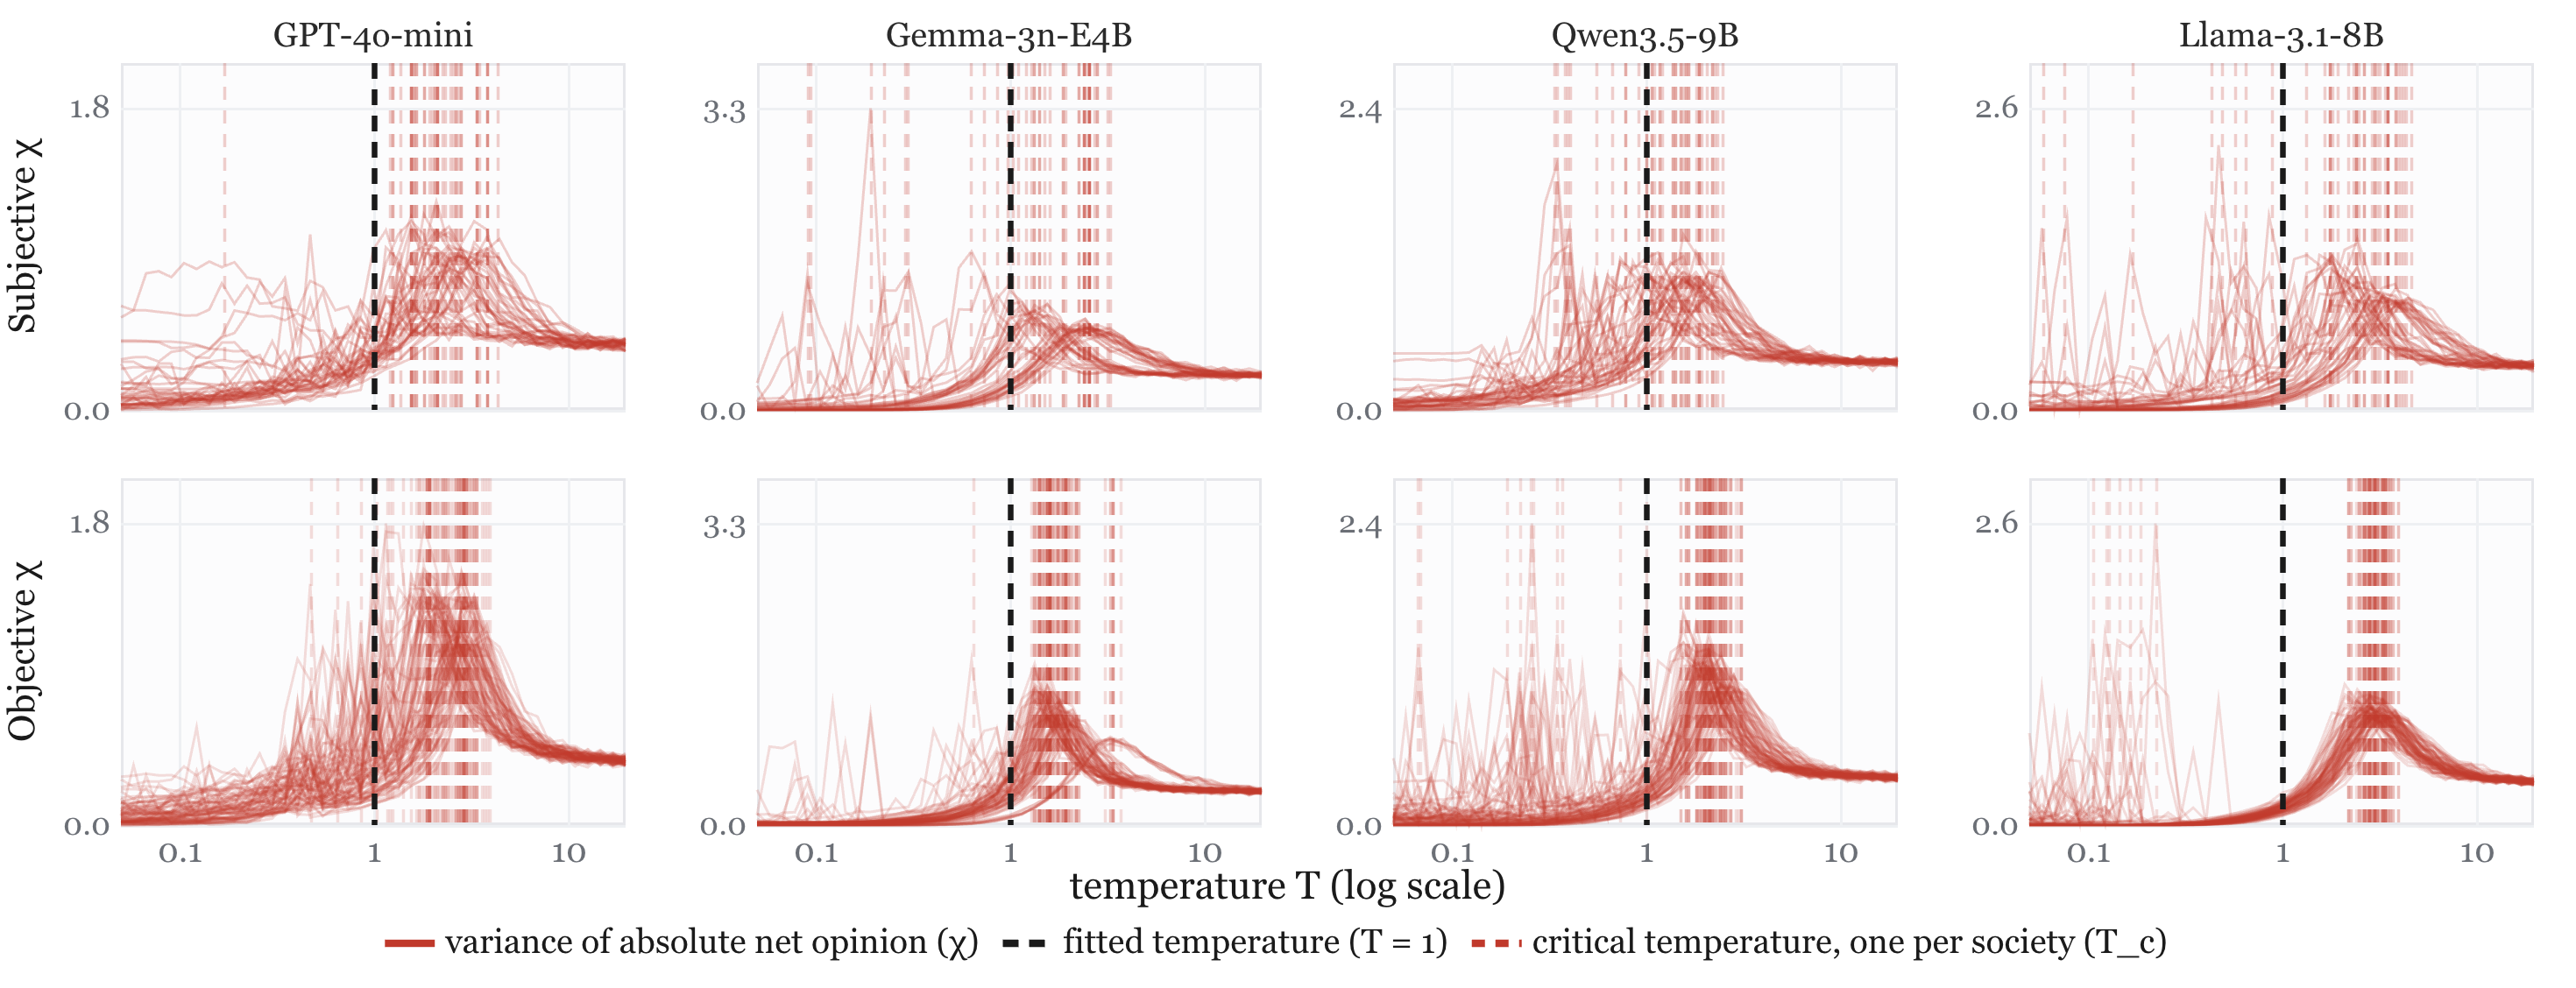
\includegraphics[width=0.99\textwidth]{main/Figures/apx_08_temperature_sweep_grid.png}
\caption{\textit{Figure~\ref{fig:agent_model_tc_mean_test_J03_fitted_nomf_tcmean} with each question-$J$ pair presented individually.} Figure~\ref{fig:agent_model_tc_mean_test_J03_fitted_nomf_tcmean} in
Section~\ref{sec:results_temperature} reports the across-community mean of these curves and the
across-community mean of their $\chi$-peak $\mathcal{T}_c$'s. This figure shows the same sweep without any
averaging with one curve and one $\mathcal{T}_c$ line per group. \label{fig:agent_model_tc_mean_test_J03_fitted_nomf_tcmean_qea}}
\end{figure}





This appendix explains how the critical temperatures in Section~\ref{sec:results_temperature} are computed. To avoid confusion, we begin by clarifying that this experiment does not modify the language model’s temperature. Instead, it modifies the temperature of the fitted model, as described below.

\textit{Setup.} The experiment covers every question in the test set and four in-distribution random graphs. Four graphs $\times$ the test question bank gives $80$
objective and $40$ subjective groups per model, each with four independent episodes. 

\textit{Model.} The sweep uses the parameters of the three-coupling discrete update rule.

\textit{Introducing Temperature.} Our fitted rule is
$P\big(s_i(t{+}1)=+1\big) = \sigma\big(h_i\big)$. Reintroducing the temperature divides that
logit by $\mathcal{T}$,
\[
P\big(s_i = +1\big) \;=\; \sigma\!\left(\frac{h_i}{\mathcal{T}}\right),
\]
so the $\mathcal{T}=1$ point of the sweep is the fitted model itself.

\textit{Initialization.} We call a $J$ paired with a question a \textit{group}. For each group, we have taken $4$ independent trajectories in our experiments. The $4$ trajectories are considered as the different rollouts of the same system in the temperature sweep as well. We initialize a group at each of the four starting points at $t=0$ from the $4$ independently sampled trajectories.  

\textit{Procedure.} We sweep $41$ log-spaced temperatures from $0.05$ to $20$.\footnote{$0.050, 0.058, 0.067, 0.078, 0.091, 0.106, 0.123, 0.143, 0.166, 0.193, 0.224, 0.260, 0.302, 0.350, 0.407, 0.473, 0.549, 0.638, 0.741, 0.861, 1.000,\\ 1.162, 1.349, 1.567, 1.821, 2.115, 2.456, 2.853, 3.314, 3.850, 4.472, 5.195, 6.034, 7.009, 8.142, 9.457, 10.986, 12.761, 14.823, 17.218, 20.000
$} At each
temperature, we run the model for $500$ synchronous steps. We discard the first $200$ (to account for the time it takes for the community to reach equilibrium) and retain the last $300$. During this run, each agent's opinion in the next step $s_i = \pm1$ is sampled with probability $\sigma(h_i/\mathcal{T})$.

\textit{Observables.} From the $300$ steps of the group trajectories, we compute $\chi \;=\; N\,\mathrm{Var}_t\big(|n(t)|\big)$. The four independent trajectories per group are used as four independent initial conditions that are then averaged into one $\chi$ curve per group.

\textit{Locating $\mathcal{T}_c$.} A group's $\mathcal{T}_c$ is the location of its $\chi$ peak. Since the grid is
coarse relative to the width of the peak, we fit a parabola through the maximizing
grid point and its two neighbors in $\log \mathcal{T}$ and take the vertex, which resolves $\mathcal{T}_c$ below the
spacing of the $41$-point grid.
